\begin{table} [h]
\begin{center}
\begin{tabular}{|c|c|}
	\hline
	$Номер результата измерений j$ & $Результат измерений x_j$\\
	\hline
	1 & -2.46 \\ \hline
2 & -2.10 \\ \hline
3 & -1.16 \\ \hline
4 & -1.04 \\ \hline
5 & -0.99 \\ \hline
6 & -0.92 \\ \hline
7 & -0.91 \\ \hline
8 & -0.71 \\ \hline
9 & -0.66 \\ \hline
10 & -0.38 \\ \hline
11 & -0.27 \\ \hline
12 & -0.22 \\ \hline
13 & -0.18 \\ \hline
14 & -0.09 \\ \hline
15 & -0.06 \\ \hline
16 & 0.01 \\ \hline
17 & 0.082 \\ \hline
18 & 0.10 \\ \hline
19 & 0.16 \\ \hline
20 & 0.22 \\ \hline
21 & 0.32 \\ \hline
22 & 0.37 \\ \hline
23 & 0.43 \\ \hline
24 & 0.45 \\ \hline
25 & 0.52 \\ \hline
26 & 0.63 \\ \hline
27 & 0.76 \\ \hline
28 & 1.83 \\ \hline
29 & 1.97 \\ \hline
30 & 2.44 \\ \hline
\end{tabular}
\end{center}
\caption{Результаты измерений, упорядоченные по значению, n = 30}
\end{table} 

\begin{figure}[h]
\center{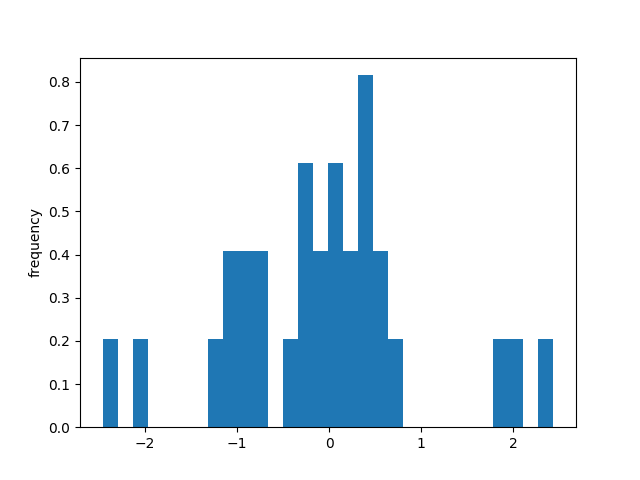
\includegraphics[width=1\linewidth]{normCramer30.png}}
\caption{Пробная выборка, n = 30}
\label{fig:box20}
\end{figure}


\begin{table} [h]
\resizebox{0.7\textwidth}{!}{\begin{minipage}{\textwidth}
\begin{tabular}{|c|c|c|c|c|c|c|c|c|c|}
	\hline
	$j$ & $A_j=\frac{2j-1}{2n}$ & $B_j=F(x_j)$  & $C_j=ln(B_j)$ & $D_j=(A_j)(C_j)$ & $E_j=1-A_j$ & $F_j=1-B_j$ & $G_j=ln(F_j))$ & $H_j=(E_j)(G_j)$ & $I_j=(D_j)+(H_j)$\\
	\hline
	 1 &  0.017 &  0.011222 &  -4.48988 &  -0.07483 &  0.9833 &  0.988778 &  -0.01129 &  -0.01110 &  -0.08593 \\ \hline
2 &  0.050 &  0.025776 &  -3.65829 &  -0.18291 &  0.9500 &  0.974224 &  -0.02611 &  -0.02481 &  -0.20772 \\ \hline
3 &  0.083 &  0.146270 &  -1.92230 &  -0.16019 &  0.9167 &  0.853730 &  -0.15814 &  -0.14496 &  -0.30515 \\ \hline
4 &  0.117 &  0.175266 &  -1.74145 &  -0.20317 &  0.8833 &  0.824734 &  -0.19269 &  -0.17021 &  -0.37338 \\ \hline
5 &  0.150 &  0.187294 &  -1.67507 &  -0.25126 &  0.8500 &  0.812706 &  -0.20739 &  -0.17628 &  -0.42754 \\ \hline
6 &  0.183 &  0.205472 &  -1.58245 &  -0.29012 &  0.8167 &  0.794528 &  -0.23001 &  -0.18784 &  -0.47795 \\ \hline
7 &  0.217 &  0.209139 &  -1.56476 &  -0.33903 &  0.7833 &  0.790861 &  -0.23463 &  -0.18380 &  -0.52283 \\ \hline
8 &  0.250 &  0.268296 &  -1.31566 &  -0.32892 &  0.7500 &  0.731704 &  -0.31238 &  -0.23428 &  -0.56320 \\ \hline
9 &  0.283 &  0.282907 &  -1.26264 &  -0.35775 &  0.7167 &  0.717093 &  -0.33255 &  -0.23833 &  -0.59607 \\ \hline
10 &  0.317 &  0.378800 &  -0.97075 &  -0.30740 &  0.6833 &  0.621200 &  -0.47610 &  -0.32534 &  -0.63274 \\ \hline
11 &  0.350 &  0.419482 &  -0.86873 &  -0.30406 &  0.6500 &  0.580518 &  -0.54384 &  -0.35349 &  -0.65755 \\ \hline
12 &  0.383 &  0.439694 &  -0.82168 &  -0.31498 &  0.6167 &  0.560306 &  -0.57927 &  -0.35722 &  -0.67219 \\ \hline
13 &  0.417 &  0.452555 &  -0.79285 &  -0.33035 &  0.5833 &  0.547445 &  -0.60249 &  -0.35145 &  -0.68181 \\ \hline
14 &  0.450 &  0.487318 &  -0.71884 &  -0.32348 &  0.5500 &  0.512682 &  -0.66810 &  -0.36745 &  -0.69093 \\ \hline
15 &  0.483 &  0.497777 &  -0.69760 &  -0.33717 &  0.5167 &  0.502223 &  -0.68871 &  -0.35583 &  -0.69301 \\ \hline
16 &  0.517 &  0.524544 &  -0.64523 &  -0.33337 &  0.4833 &  0.475456 &  -0.74348 &  -0.35935 &  -0.69272 \\ \hline
17 &  0.550 &  0.557874 &  -0.58362 &  -0.32099 &  0.4500 &  0.442126 &  -0.81616 &  -0.36727 &  -0.68826 \\ \hline
18 &  0.583 &  0.565397 &  -0.57023 &  -0.33263 &  0.4167 &  0.434603 &  -0.83332 &  -0.34722 &  -0.67985 \\ \hline
19 &  0.617 &  0.586767 &  -0.53313 &  -0.32876 &  0.3833 &  0.413233 &  -0.88374 &  -0.33877 &  -0.66753 \\ \hline
20 &  0.650 &  0.606438 &  -0.50015 &  -0.32510 &  0.3500 &  0.393562 &  -0.93252 &  -0.32638 &  -0.65148 \\ \hline
21 &  0.683 &  0.644371 &  -0.43948 &  -0.30031 &  0.3167 &  0.355629 &  -1.03387 &  -0.32739 &  -0.62770 \\ \hline
22 &  0.717 &  0.662093 &  -0.41235 &  -0.29552 &  0.2833 &  0.337907 &  -1.08499 &  -0.30741 &  -0.60293 \\ \hline
23 &  0.750 &  0.680732 &  -0.38459 &  -0.28844 &  0.2500 &  0.319268 &  -1.14173 &  -0.28543 &  -0.57387 \\ \hline
24 &  0.783 &  0.687730 &  -0.37436 &  -0.29325 &  0.2167 &  0.312270 &  -1.16389 &  -0.25218 &  -0.54542 \\ \hline
25 &  0.817 &  0.712201 &  -0.33940 &  -0.27717 &  0.1833 &  0.287799 &  -1.24549 &  -0.22834 &  -0.50551 \\ \hline
26 &  0.850 &  0.747836 &  -0.29057 &  -0.24699 &  0.1500 &  0.252164 &  -1.37767 &  -0.20665 &  -0.45364 \\ \hline
27 &  0.883 &  0.784050 &  -0.24328 &  -0.21490 &  0.1167 &  0.215950 &  -1.53271 &  -0.17882 &  -0.39372 \\ \hline
28 &  0.917 &  0.964333 &  -0.03632 &  -0.03329 &  0.0833 &  0.035667 &  -3.33352 &  -0.27779 &  -0.31109 \\ \hline
29 &  0.950 &  0.973784 &  -0.02657 &  -0.02524 &  0.0500 &  0.026216 &  -3.64139 &  -0.18207 &  -0.20731 \\ \hline
30 &  0.983 &  0.991406 &  -0.00863 &  -0.00849 &  0.0167 &  0.008594 &  -4.75673 &  -0.07928 &  -0.08777 \\ \hline
	$\sum$ & & & & & & & & & -15.2768\\
	\hline
\end{tabular}
\end{minipage} }
\caption{Результаты промежуточных вычислений значения статистики $n\Omega_n^2$ по формуле \ref{eq:Г1}, n = 30} \label{tab:nomega} 
\end{table} 